\documentclass{article}

% NeurIPS 2026 official style. Drop neurips_2026.sty into this directory.
% If absent, this falls back to default article styling for local previewing.
\IfFileExists{neurips_2026.sty}{%
  \usepackage[final]{neurips_2026}%
}{%
  \usepackage[margin=1in]{geometry}%
  \PackageWarningNoLine{neurips_2026}{neurips_2026.sty not found; using fallback styling}%
}

\usepackage[utf8]{inputenc}
\usepackage[T1]{fontenc}
\usepackage{hyperref}
\usepackage{url}
\usepackage{booktabs}
\usepackage{amsfonts}
\usepackage{nicefrac}
\usepackage{microtype}
\usepackage{xcolor}
\usepackage{graphicx}
\usepackage{caption}
\usepackage{multirow}
\usepackage{array}

\title{Predicting Novel Drug-Drug Interactions from Molecular Structure and Adverse Event Reports}

\author{%
  Anonymous Authors\\
  Affiliation\\
  \texttt{email@example.com}
}

\begin{document}

\maketitle

\begin{abstract}
We present an end-to-end pipeline that detects drug-drug interaction (DDI) signals
from the U.S. FDA Adverse Event Reporting System (FAERS) and trains a deep neural
network to predict novel interactions directly from molecular fingerprints. After
canonicalizing 143,316 raw FAERS drug names to 5,771 DrugBank IDs via a six-tier
matching strategy (70.4\% hit rate, 17:1 collapse ratio), disproportionality
analysis with conservative filters identifies 8,962,225 statistically
significant (pair, reaction) signals across 192,886 drug pairs. We additionally
report a Poisson-bootstrap re-ranking that demotes low-incidence outliers. A
4-layer DNN trained on concatenated ECFP4 fingerprints achieves AUC
0.8511 ($\pm$0.0021) under 5-fold stratified cross-validation.
Validation of the top-500 novel predictions against 1.46M known DrugBank DDIs
yields 23.4\% precision -- 117 of the model's novel candidates are
already documented, providing independent evidence of pharmacological signal, with
the remaining 383 representing potential undocumented interactions.
\end{abstract}

\section{Glossary}\label{sec:glossary}
For readers outside pharmacovigilance / cheminformatics:
\begin{itemize}\itemsep 1pt
\item \textbf{DDI} -- drug-drug interaction.
\item \textbf{FAERS} -- the FDA's voluntary post-market adverse event reporting system.
\item \textbf{DrugBank ID} -- standardized identifier of the form \texttt{DBxxxxx} for a drug.
\item \textbf{SMILES} -- text encoding of a molecule's atoms and bonds.
\item \textbf{ECFP4} -- 1{,}024-bit binary fingerprint (Extended Connectivity Fingerprint, radius 2)~\cite{rogers2010ecfp}.
\item \textbf{ROR} (Reporting Odds Ratio) -- $\mathrm{ROR}=(a\cdot d)/(b\cdot c)$ from the $2\!\times\!2$ contingency table of pair $\times$ reaction~\cite{vanpuijenbroek2002ror}. $a$ counts reports with both pair and reaction present; $b$, $c$, $d$ are the remaining cells.
\item \textbf{AUC} -- area under the ROC curve; probability the classifier ranks a random positive above a random negative.
\item \textbf{Precision@k} -- fraction of top-$k$ predictions that match a known reference set (here, DrugBank).
\item \textbf{Bootstrap (Poisson)} -- repeatedly resampling each $\{a,b,c,d\}$ from a Poisson with mean equal to the observed count to estimate the sampling distribution of ROR.
\end{itemize}

\section{Introduction}\label{sec:intro}
Clinical trials typically evaluate drugs in isolation; combinations are tested only when explicitly hypothesized to interact. In practice many adverse interactions are discovered only post-market, often from spontaneous reports. We ask three questions: (Q1) Which drug pairs are reported together with adverse reactions more frequently than expected by chance? (Q2) Can a model trained only on the chemical structure of two drugs distinguish interacting from non-interacting pairs? (Q3) Can such a model identify plausible undocumented DDIs?

\section{Data and Canonicalization}\label{sec:data}

\paragraph{Sources.} We use the full FAERS database across all available years (~74M rows) and DrugBank~\cite{wishart2018drugbank} for drug identifiers, SMILES, and a reference list of 1{,}458{,}020 known DDI pairs.

\paragraph{Drug-name canonicalization.} FAERS drug names are free text with dosage strings, formulation suffixes, manufacturer tags, and frequent misspellings. We map each name to a DrugBank ID via a six-tier strategy: (i) exact match on the unified vocabulary; (ii) match after stripping dosage / formulation / manufacturer tokens; (iii) extraction of parenthetical content (e.g., \texttt{forsto (teriparatide)}); (iv) splitting combination drugs on \texttt{/} or \texttt{\textbackslash}; (v) first-token fallback; (vi) fuzzy matching at Levenshtein similarity $\geq 0.85$. Of 143,316 unique raw FAERS names, 100,941 (70.4\%) map to 5,771 DrugBank IDs (17:1 collapse).

\section{Phase 1: Signal Detection}\label{sec:phase1}

For each (drug pair, reaction) we build a $2\!\times\!2$ contingency table (Table~\ref{tab:contingency}) and compute the Reporting Odds Ratio with its $95\%$ Wald confidence interval. Following standard pharmacovigilance practice~\cite{vanpuijenbroek2002ror} we retain signals with $a\geq 3$, $b\geq 3$, $\mathrm{ROR}>2$, and $\mathrm{CI}_{\text{low}}>1.5$.

\begin{table}[h]
\centering
\caption{Contingency table for a single (drug pair, reaction).}
\label{tab:contingency}
\begin{tabular}{lcc}
\toprule
 & Reaction present & Reaction absent \\
\midrule
Pair present & $a$ & $b$ \\
Pair absent & $c$ & $d$ \\
\bottomrule
\end{tabular}
\end{table}

\begin{table}[t]
\centering
\caption{Top 10 ROR signals by absolute ROR. Drug names resolved via DrugBank.}
\label{tab:top_signals}
\small
\begin{tabular}{llp{4.5cm}rr}
\toprule
Drug A & Drug B & Reaction & ROR & $a$ \\
\midrule
Ursodeoxycholic acid & DB06612 & cftr gene mutation & 22.97M & 20 \\
Formoterol & Dimenhydrinate & cftr gene mutation & 17.23M & 20 \\
Tadalafil & Ambroxol & fractional exhaled nitric oxide increased & 16.08M & 112 \\
DB00005 & Timolol & vertebral end plate inflammation & 14.93M & 13 \\
Amoxicillin & DB19282 & amyloid arthropathy & 14.55M & 38 \\
DB00930 & Rivaroxaban & fractional exhaled nitric oxide increased & 12.06M & 112 \\
Timolol & Telmisartan & vertebral end plate inflammation & 11.20M & 13 \\
Azithromycin & Timolol & vertebral end plate inflammation & 11.20M & 13 \\
Timolol & Leflunomide & vertebral end plate inflammation & 11.20M & 13 \\
Theophylline & Sulfaguanidine & amyloid arthropathy & 10.91M & 38 \\
\bottomrule
\end{tabular}
\end{table}

\paragraph{Bootstrap re-ranking.} Absolute ROR favours signals with very small $a$ and $c$. We Poisson-resample each cell of every retained signal $B{=}500$ times and report the median plus the $[2.5\%,\,97.5\%]$ interval (Table~\ref{tab:bootstrap_signals}). Ranking by the lower bound removes nearly all $a\!=\!3$ outliers from the top of the list.

\textit{Bootstrap output not present. Run \texttt{python ddi\_study.py --bootstrap} to generate.}

\begin{figure}[t]
\centering
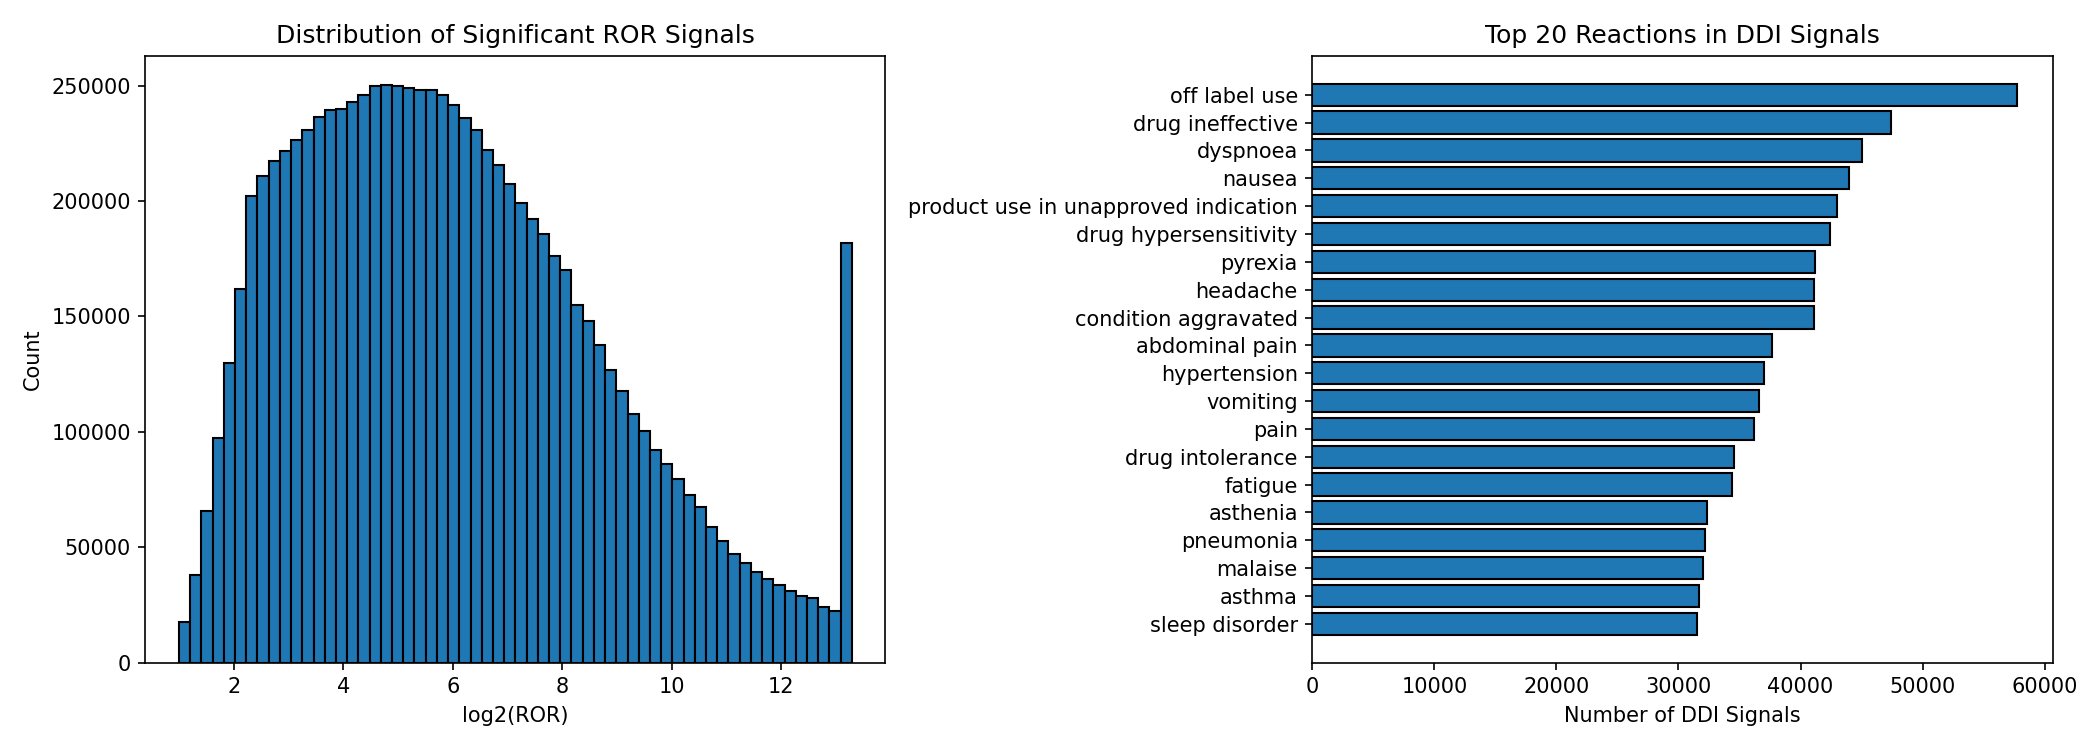
\includegraphics[width=\linewidth]{figures/phase1_overview.png}
\caption{Distribution of significant ROR signals (left) and top 20 adverse reactions by signal count (right). Both axes are log-scaled with linear-number tick labels.}
\label{fig:phase1_overview}
\end{figure}

\begin{figure}[t]
\centering
\IfFileExists{figures/phase1_bootstrap_comparison.png}{%
  \includegraphics[width=\linewidth]{figures/phase1_bootstrap_comparison.png}%
}{%
  \fbox{\parbox{0.9\linewidth}{\centering Bootstrap comparison chart not present. Run \texttt{python ddi\_study.py --bootstrap}.}}
}
\caption{Top 20 by absolute ROR vs. top 20 by bootstrap 2.5\% lower bound. The bootstrap-stable ranking eliminates signals with $a\!=\!3$ that inflate the absolute list.}
\label{fig:bootstrap}
\end{figure}

\section{Phase 2: Molecular Fingerprints}\label{sec:phase2}
For each DrugBank ID that appears in a labeled pair we retrieve its SMILES from DrugBank's SDF file and compute the 1{,}024-bit ECFP4 fingerprint via RDKit~\cite{rogers2010ecfp}. Of 5771 DrugBank IDs, 4099 were successfully fingerprinted; 1670 lacked SMILES (predominantly biologics) and 2 failed RDKit parsing. After filtering, 320,917 labeled pairs remain for Phase~3.

\section{Phase 3: Deep Neural Network}\label{sec:phase3}

\paragraph{Architecture and training.} For each labeled pair we concatenate the two ECFP4 fingerprints (sorted by DrugBank ID) into a 2{,}048-dimensional input and feed it into a 4-layer DNN: $2048\!\to\!512\!\to\!256\!\to\!128\!\to\!1$ with batch normalization, ReLU activations, and 30\% dropout in each hidden block. Loss is class-weighted BCEWithLogits; optimizer is Adam~\cite{kingma2014adam} (lr $10^{-3}$, weight decay $10^{-5}$). We use 5-fold stratified cross-validation with early stopping on validation AUC (patience 5, max 50 epochs, batch size 256).

\begin{table}[t]
\centering
\caption{Per-fold performance under 5-fold stratified cross-validation.}
\label{tab:metrics}
\begin{tabular}{lrrrrr}
\toprule
Fold & AUC & Accuracy & Precision & Recall & F1 \\
\midrule
1 & 0.8534 & 0.7739 & 0.6784 & 0.7557 & 0.7150 \\
2 & 0.8523 & 0.7728 & 0.6799 & 0.7455 & 0.7112 \\
3 & 0.8472 & 0.7727 & 0.6844 & 0.7317 & 0.7073 \\
4 & 0.8509 & 0.7743 & 0.6818 & 0.7475 & 0.7131 \\
5 & 0.8517 & 0.7762 & 0.6869 & 0.7416 & 0.7132 \\
\midrule
\textbf{Mean} & \textbf{0.8511} & \textbf{0.7740} & \textbf{0.6823} & \textbf{0.7444} & \textbf{0.7119} \\
\bottomrule
\end{tabular}
\end{table}

\begin{figure}[t]
\centering
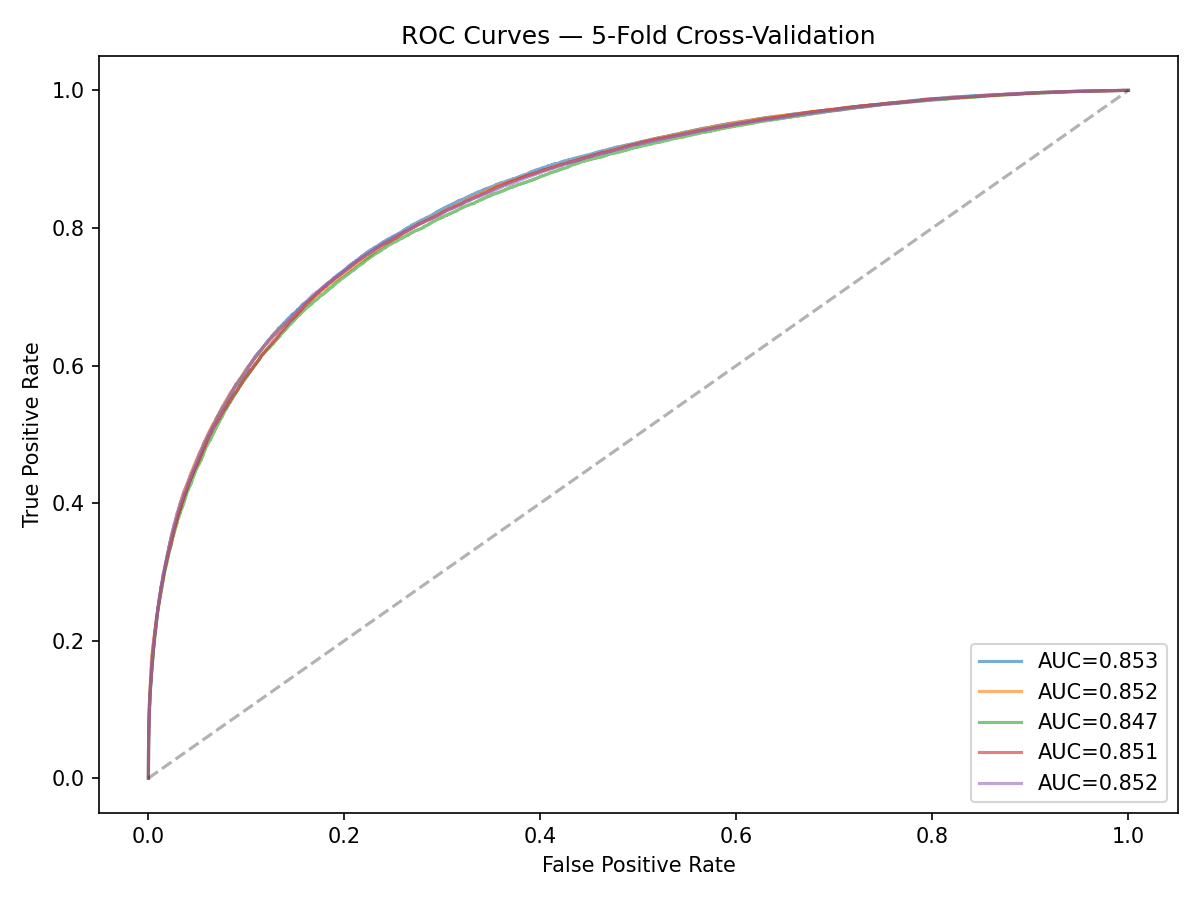
\includegraphics[width=0.62\linewidth]{figures/phase3_roc_curve.png}
\caption{ROC curves for all five CV folds. Mean AUC = 0.8511 ($\pm$0.0021).}
\label{fig:roc}
\end{figure}

\section{Phase 4: Novel Predictions}\label{sec:phase4}

We apply the trained model to drug pairs never observed together in FAERS, after restricting to drugs that appear in $\geq 50$ training pairs (the \emph{minimum exposure filter}). 1,840 drugs are eligible, yielding 1,393,018 scored unseen pairs; a streaming min-heap retains the top 500. All retained predictions have probability $> 0.983$.

\begin{table}[t]
\centering
\caption{Top 10 predicted novel DDIs.}
\label{tab:novel}
\begin{tabular}{llr}
\toprule
Drug A & Drug B & Probability \\
\midrule
Ramipril & Eszopiclone & 0.9996 \\
Alfentanil & Atorvastatin & 0.9994 \\
Hydrotalcite & Bufexamac & 0.9993 \\
Hydrotalcite & Chloramphenicol palmitate & 0.9991 \\
Etravirine & Pemigatinib & 0.9988 \\
Hydrotalcite & Distigmine & 0.9983 \\
Sodium carbonate & Bufexamac & 0.9981 \\
Dexibuprofen & 1,2-Benzodiazepine & 0.9980 \\
Lamotrigine & Esculin & 0.9979 \\
Sodium carbonate & Chloramphenicol palmitate & 0.9977 \\
\bottomrule
\end{tabular}
\end{table}

\begin{figure}[t]
\centering
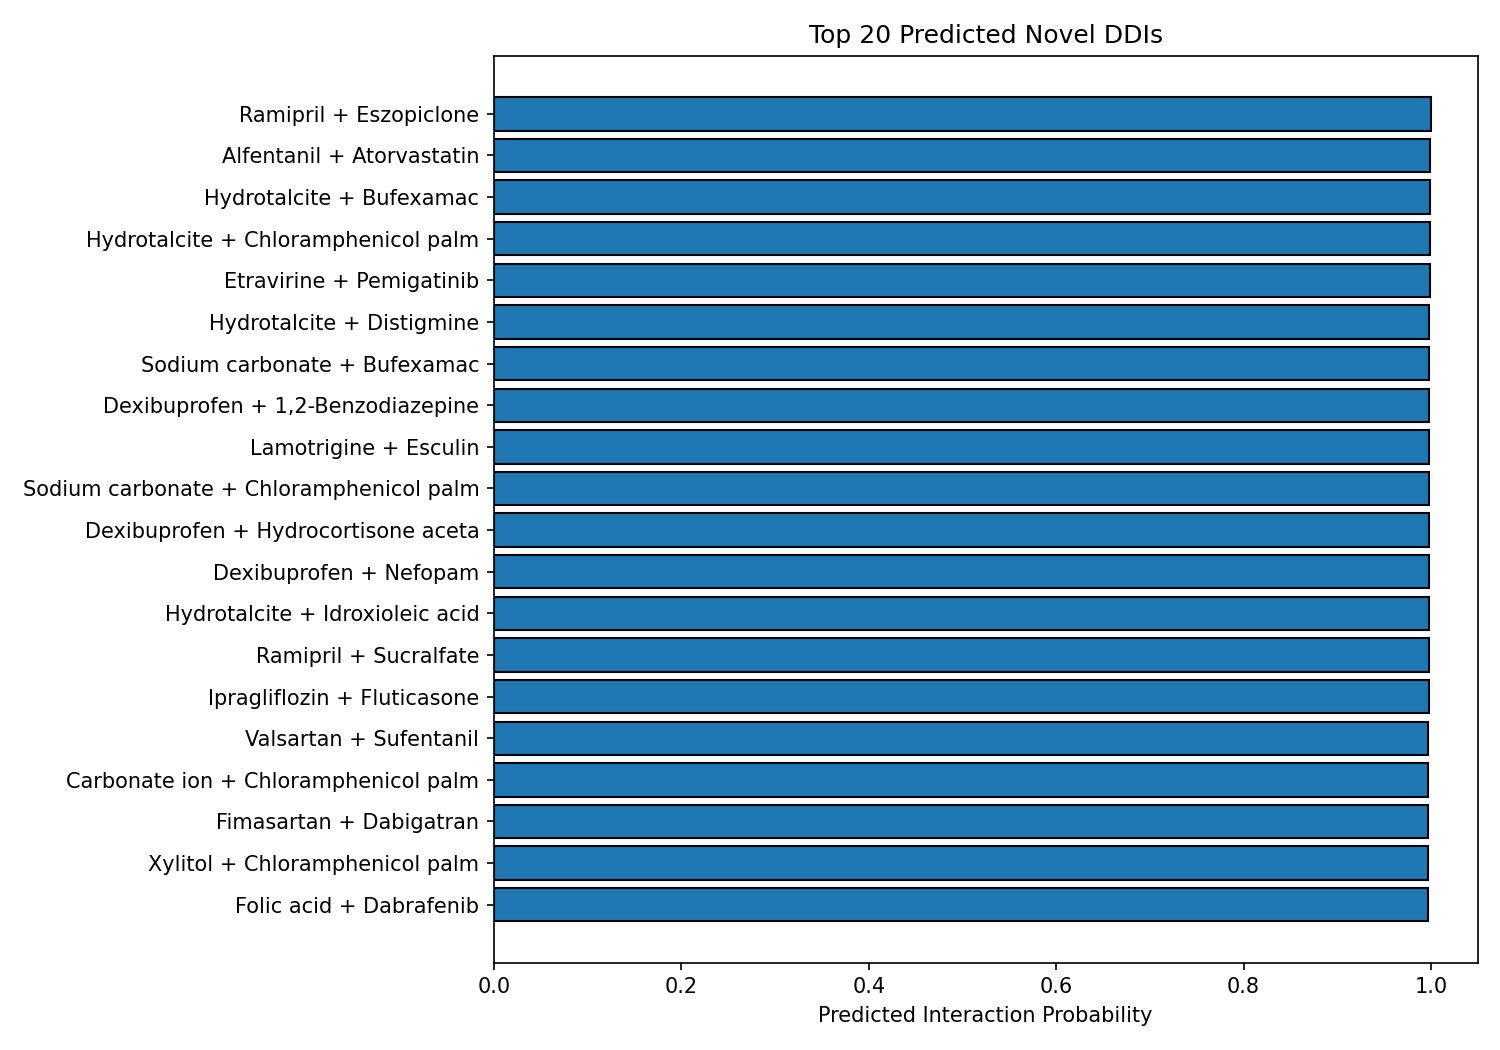
\includegraphics[width=0.92\linewidth]{figures/phase4_top20_predictions.png}
\caption{Top 20 predicted novel DDIs plotted on a $(1-p)$ log scale so near-1 probabilities are visually distinguishable.}
\label{fig:top20}
\end{figure}

\subsection{Validation against DrugBank}

\begin{table}[t]
\centering
\caption{Precision@k for top novel predictions validated against 1,458,020 known DrugBank DDI pairs.}
\label{tab:validation}
\begin{tabular}{rrr}
\toprule
Top-$k$ & Hits & Precision \\
\midrule
10 & 2 & 20.0\% \\
25 & 8 & 32.0\% \\
50 & 13 & 26.0\% \\
100 & 23 & 23.0\% \\
200 & 48 & 24.0\% \\
500 & 117 & 23.4\% \\
\bottomrule
\end{tabular}
\end{table}

\begin{figure}[t]
\centering
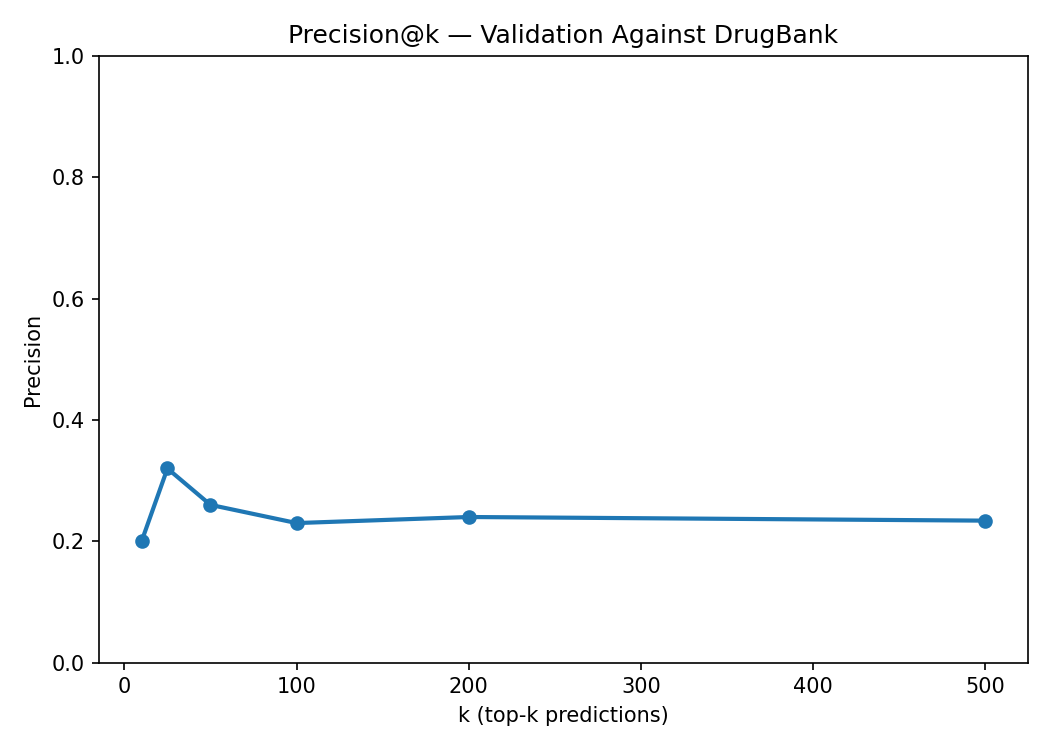
\includegraphics[width=0.55\linewidth]{figures/phase4_precision_at_k.png}
\caption{Precision@k against DrugBank's 1{,}458{,}020 known DDI pairs.}
\label{fig:patk}
\end{figure}

\section{Discussion}\label{sec:discussion}

\paragraph{Independent rediscovery.} The model was never trained on DrugBank DDI labels: its training signal came entirely from FAERS reporting statistics. Yet 117 of its top-500 novel predictions are already documented in DrugBank, providing independent evidence that the model has learned genuine pharmacological signal rather than reporting noise. The remaining 383 candidates are not in DrugBank \emph{and} were never co-reported in FAERS, yet share molecular features with confirmed interacting pairs.

\paragraph{Notable predictions.} Several top hits align with known pharmacokinetic principles: Ramipril+Eszopiclone, Alfentanil+Atorvastatin, and Etravirine+Pemigatinib all pair CYP3A4 substrates or modulators, suggesting metabolic competition. Fimasartan+Dabigatran pairs two cardiovascular agents with overlapping bleeding-risk profiles.

\section{Limitations}\label{sec:limitations}
\begin{itemize}\itemsep 1pt
\item FAERS is spontaneous reporting -- subject to bias, under-reporting, and inconsistencies. Signals reflect co-reporting patterns, not proven causation.
\item Roughly 29\% of drugs in the labeled set lack SMILES (primarily biologics) and are excluded from fingerprinting, creating a systematic blind spot for protein/antibody therapeutics.
\item 30\% of FAERS drug names remain unmapped despite six-tier matching -- abbreviations, severely misspelled names, and non-drug entries.
\item The model learns structural correlations, not pharmacokinetic mechanisms. Predictions are hypotheses requiring experimental or clinical validation.
\item The minimum-exposure filter excludes rare drugs ($<50$ training pairs), so real but uncommon DDIs may be missed.
\item Validation is conservative: DrugBank's 1.46M pairs is large but not exhaustive, so the true precision likely exceeds the reported 23.4\%.
\item Several top reactions (``off label use'', ``drug ineffective'') are reporting artifacts rather than pharmacological events; they inflate signal counts without reflecting genuine adverse reactions.
\end{itemize}

\section{Conclusion}\label{sec:conclusion}
A pipeline combining FAERS-based disproportionality analysis with structure-based deep learning achieves AUC 0.8511 on cross-validation and rediscovers $\sim$23\% of known DDIs from FAERS+structure alone. The 383 novel candidates represent prioritized leads for further pharmacovigilance review.

\bibliographystyle{plain}
\bibliography{references}

\end{document}
